\documentclass{standalone}
\usepackage{tikz}
\usetikzlibrary{arrows.meta}

\begin{document}
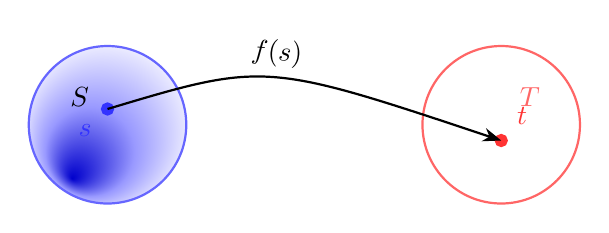
\begin{tikzpicture}[>=Stealth, thick]

  % Define a steeper radial shading (gradient) for S
  \pgfdeclareradialshading{biasedS}{\pgfpoint{-0.4cm}{-0.6cm}}%
    {%
      color(0cm)=(blue!80!black);
      color(0.5cm)=(blue!40);
      color(0.9cm)=(blue!10!white);
      color(1.0cm)=(white)
    }

  % Draw biased set S with gradient fill
  \shade[shading=biasedS, draw=blue!60, thick] (-2,0) circle (1.0cm);
  \node[above left=3pt] at (-2,0) {$S$};

  % Draw regular set T
  \draw[red!60, thick] (3,0) circle (1.0cm) node[above right=3pt] {$T$};

  % Elements s and t
  \filldraw[blue!80] (-2,0.2) circle (2pt) node[below left=2pt] {$s$};
  \filldraw[red!80]  (3,-0.2) circle (2pt) node[above right=2pt] {$t$};

  % Curved function arrow
  \draw[->, thick]
    (-2,0.2) .. controls (0,0.8) .. (3,-0.2)
    node[midway, above, sloped] {$f(s)$};

\end{tikzpicture}
\end{document}
